\documentclass[preview]{standalone}
\usepackage{amsmath}
\usepackage{amssymb}
\usepackage{stellar}
\usepackage{definitions}
\usepackage{bettelini}
\usepackage{tikz}
\usepackage{pgfplots}
\pgfplotsset{compat=1.18}
\begin{document}
\id{diffeq-qualitative-analysis-exercises}
\genpage
\section{Exercises}

\begin{snippetexercise}{diffeq-arctan-cube-root-exercise}{Local and global uniqueness}
    Let \(g(y)=\sqrt[3]{\arctan(y^2-y)}\), using the real cube root,
    and consider \(P_{a,b}\colon y'=xg(y)\), \(y(a)=b\).
    Show global existence, construct at least nine solutions of \(P_{0,1}\),
    and discuss uniqueness for \(P_{a,1}\), \(P_{0,b}\) and \(P_{1,b}\).
\end{snippetexercise}

\begin{snippetsolution}{diffeq-arctan-cube-root-global}{Existence and the phase diagram}
    For \(y'=x\sqrt[3]{\arctan(y^2-y)}\), continuity gives local existence and
    \[
        |f(x,y)|\leq(\pi/2)^{1/3}|x|
    \]
    gives global extension by linear growth. The equilibria are \(0,1\).
    Away from them the field is locally smooth; at them the state derivative
    is singular. Its sign is the sign of \(x\) for \(y<0\) or \(y>1\),
    and the opposite sign for \(0<y<1\).
    All solutions have \(y'(0)=0\). The original sign diagram is schematic.
\begin{center}
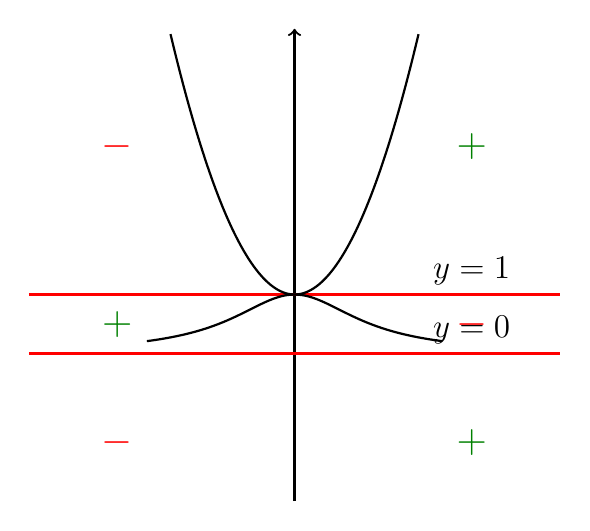
\begin{tikzpicture}[scale=0.75]
                        \draw [thick, ->] (0,-2.5) -- (0,5.5);
                        \draw [red, thick] (-4.5,0) -- (4.5,0);
                        \draw [red, thick] (-4.5,1) -- (4.5,1);
                        \draw [thick, domain=-2.1:2.1, samples=100] plot (\x, {(\x)^2 + 1});
                        \draw [thick, domain=-2.5:2.5, samples=100] plot (\x, {1/(0.6*(\x)^2 + 1)});

                        \node[above] at (3,1) {\large $y=1$};
                        \node[above] at (3,0) {\large $y=0$};

                        \node at (-3, 3.5) {\color{red} \Large $-$};
                        \node at (3, 3.5) {\color{green!50!black} \Large $+$};

                        \node at (-3, 0.5) {\color{green!50!black} \Large $+$};
                        \node at (3, 0.5) {\color{red} \Large $-$};

                        \node at (-3, -1.5) {\color{red} \Large $-$};
                        \node at (3, -1.5) {\color{green!50!black} \Large $+$};
                    \end{tikzpicture}
\end{center}
\end{snippetsolution}

\begin{snippetsolution}{diffeq-arctan-cube-root-nine}{Nine choices and waiting times}
    For \(g(y)=\sqrt[3]{\arctan(y^2-y)}\), put
    \[
        H(y)=\int_1^y\frac{dt}{g(t)}.
    \]
    On each side of \(1\), this is positive. The singularities at \(0\) and
    \(1\) are integrable because \(g(t)\sim-\sqrt[3]t\) at \(0^+\), and
    \(g(t)\sim\sqrt[3]{t-1}\) at \(1\).
    Nonconstant branches through \((0,1)\) satisfy
    \[
        H(y)=x^2/2,\qquad x=\pm\sqrt{2H(y)}.
    \]
    On each half-axis one may stay at \(1\), enter \(y>1\), or enter \(0<y<1\).
    These choices are independent, giving nine solutions, and arbitrary
    waiting times give infinitely many more. For departure at \(|x|=c\),
    use \(H(y)=(x^2-c^2)/2\) on that side.
    The lower branch reaches zero at finite time, since \(H(0)<\infty\),
    and must then remain there in the outward time direction.
    The upper branch cannot have a finite horizontal asymptote: such a limit
    would give bounded \(H\) while \(x^2/2\to\infty\).
    Since \(g(y)\to(\pi/2)^{1/3}\),
    \[
        y(x)\sim\frac{(\pi/2)^{1/3}}2x^2
    \]
    on an upper branch as \(|x|\to\infty\).
    The nine sketches retain the original waiting interval and schematic shapes.
\begin{center}
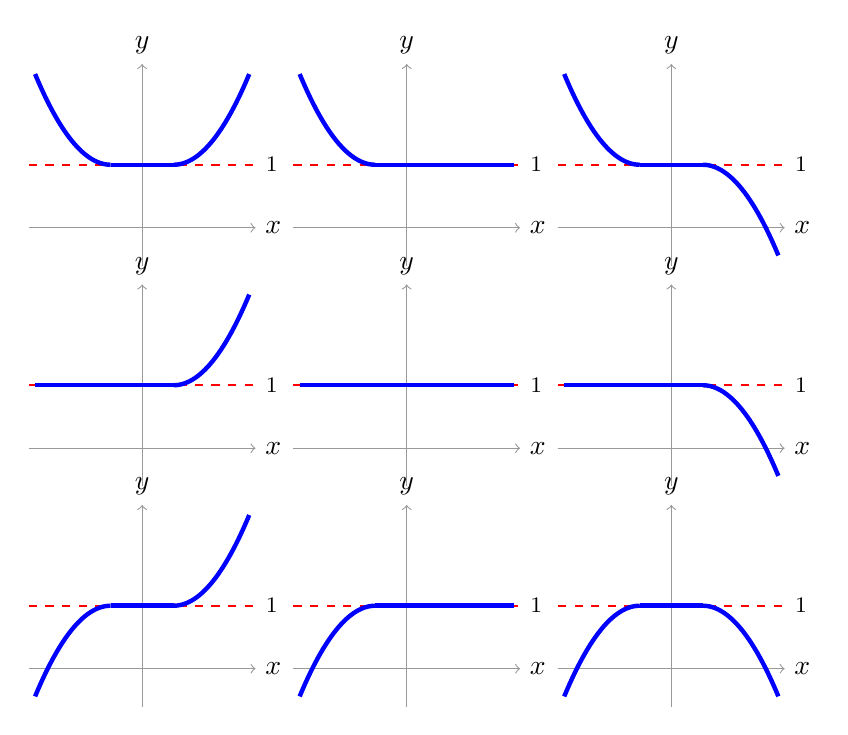
\begin{tikzpicture}[scale=0.8]
                    \foreach \i/\lfunc in {
                        0/{pow(\x+0.5, 2) + 1},
                        1/{1},
                        2/{-pow(\x+0.5, 2) + 1}%
                    } {
                        \foreach \j/\rfunc in {
                            0/{pow(\x-0.5, 2) + 1},
                            1/{1},
                            2/{-pow(\x-0.5, 2) + 1}%
                        } {
                            \begin{scope}[shift={({\j*4.2}, {-\i*3.5})}]
                                \draw[->, gray!80] (-1.8, 0) -- (1.8, 0) node[right, text=black] {$x$};
                                \draw[->, gray!80] (0, -0.6) -- (0, 2.6) node[above, text=black] {$y$};
                                \draw[red, thick, dashed] (-1.8, 1) -- (1.8, 1) node[right, text=black] {\footnotesize $1$};

                                \draw[ultra thick, blue] (-0.5, 1) -- (0.5, 1);
                                \draw[ultra thick, blue, domain=-1.7:-0.5, samples=30] plot (\x, {\lfunc});
                                \draw[ultra thick, blue, domain=0.5:1.7, samples=30] plot (\x, {\rfunc});
                            \end{scope}
                        }
                    }
                \end{tikzpicture}
\end{center}
\end{snippetsolution}

\begin{snippetsolution}{diffeq-arctan-cube-root-uniqueness}{The three uniqueness questions}
    Let \(g(y)=\sqrt[3]{\arctan(y^2-y)}\).
    For every \(a\), \(P_{a,1}\) is nonunique: besides the equilibrium,
    a branch can depart in the direction where \(x^2>a^2\), according to
    \[
        \int_1^{y(x)}\frac{dt}{g(t)}=\frac{x^2-a^2}{2}.
    \]
    At \(a=0\) the two sides are independent; at \(a\neq0\) this already
    gives nonuniqueness in every two-sided neighborhood.

    For \(P_{0,b}\), global uniqueness holds exactly when \(b\neq1\).
    If \(b>1\), the state increases outward and never reaches \(1\).
    If \(b<0\) or \(0<b<1\), it moves toward \(0\) as \(|x|\) increases.
    After reaching \(0\), the signs on both sides force it to stay there.
    At \(b=0\) the only solution is zero. Local uniqueness away from
    \(0,1\) alone would not justify these global conclusions.

    For \(P_{1,b}\), define \(b_-\in(0,1)\) and \(b_+>1\) by
    \[
        H(b_-)=H(b_+)=\frac12,\qquad H(y)=\int_1^y\frac{dt}{g(t)}.
    \]
    These points exist uniquely: \(H\) decreases from \(H(0)>1/2\) to \(0\)
    on \((0,1)\), and increases from \(0\) to infinity on \((1,\infty)\).
    Indeed \(H(0)\geq4^{1/3}>1/2\), since
    \(|g(t)|\leq(1/4)^{1/3}\) for \(0<t<1\).
    The problem has a unique global solution exactly when
    \[
        b\notin\{0\}\cup[b_-,b_+].
    \]
    For \(b\in[b_-,b_+]\), the branch traced from time \(1\) reaches \(1\)
    at some time in \([0,1]\), after which backward choices create distinct extensions.
    The threshold values are included: arrival at time zero still allows
    independent choices on the negative half-axis.
    For \(b=0\), distinct arriving branches and the zero solution give nonuniqueness.
    Outside this set, the branch remains away from \(1\) when traced to zero;
    any later outward contact with \(0\) has the forced constant continuation.
    Local uniqueness at the initial point holds for every \(b\neq0,1\);
    it must not be confused with uniqueness of a global extension.
\end{snippetsolution}

\begin{snippetexercise}{diffeq-log-root-exercise}{A state-domain boundary}
    Study \(y'=x\sqrt{|\ln y|}\), \(y>0\), including equilibria,
    possible joins, convexity and how branches approach the boundary \(y=0\).
\end{snippetexercise}

\begin{snippetsolution}{diffeq-log-root-solution}{Phase curves and contact with the boundary}
    The only equilibrium is \(y=1\), and \(y'\) has the sign of \(x\) off it.
    Reflection gives reflected solutions, but not all solutions are even:
    nonunique choices at \(1\) may differ on the two sides.
    Set
    \[
        F(y)=\int_1^y\frac{dt}{\sqrt{|\ln t|}}.
    \]
    Its singularity at \(1\) is integrable, since \(\ln t\sim t-1\).
    A nonconstant branch through \((x_0,1)\) satisfies
    \[
        F(y)=\frac{x^2-x_0^2}{2},\qquad
        x=\pm\sqrt{x_0^2+2F(y)}.
    \]
    Finite-time contact with \(1\) and waiting-time joins are possible.
    For data \(y(0)>1\), the solution stays above \(1\), is unique and global:
    \(F(y)\to+\infty\) as \(y\to+\infty\), because
    \(1/\sqrt{\ln y}\geq1/y\) eventually.
    It is strictly convex there, since
    \[
        y''=\sqrt{\ln y}+\frac{x^2}{2y}>0.
    \]
    For initial times other than zero, an initially upper branch can reach \(1\)
    backward in time, so global uniqueness needs a separate check.
    The full-strip growth theorem cannot be applied directly: the state domain
    is \(y>0\), and the field is unbounded near its boundary.

    For \(0<y<1\), put \(G(y)=\int_0^y dt/\sqrt{-\ln t}\), which is finite.
    The branches approaching \((0,0)\) satisfy \(G(y)=x^2/2\).
    They are defined on either side of zero, not at zero itself.
    Differentiating the inverse on the positive side gives
    \[
        x'(y)=\frac{1/\sqrt{-\ln y}}{\sqrt{2G(y)}},\qquad
        x'(y)^2=\frac{1/(-\ln y)}{2G(y)}.
    \]
    By l'Hopital's rule,
    \[
        \lim_{y\to0^+}x'(y)^2
        =\lim_{y\to0^+}\frac{1}{2y(-\ln y)^{3/2}}=+\infty.
    \]
    Hence \(y'(x)\to0\) at this boundary point.
    Equivalently \(G(y)\sim y/\sqrt{-\ln y}\), so
    \(x\sqrt{-\ln y}\to0\).
    At any boundary contact \((x_*,0)\) with \(x_*\neq0\), however,
    \(|y'|=|x|\sqrt{-\ln y}\to\infty\): the tangent is vertical.
    These are boundary endpoints, not intersections of classical solutions at \(y=0\).
    Below \(1\), \(y''=\sqrt{-\ln y}-x^2/(2y)\), determining changes of concavity.
    The original figure is a schematic phase sketch.
\begin{center}
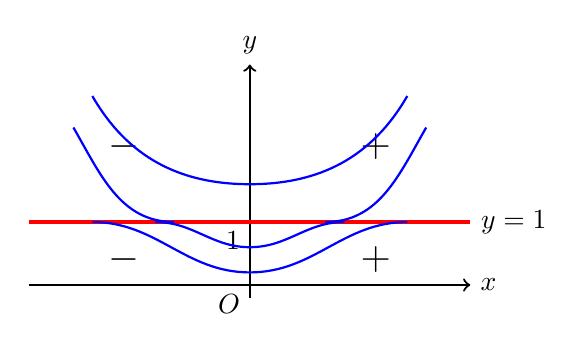
\begin{tikzpicture}[scale=0.8]
                \draw[->, thick] (-3.5, 0) -- (3.5, 0) node[right] {$x$};
                \draw[->, thick] (0, -0.2) -- (0, 3.5) node[above] {$y$};
                \node[below left] at (0,0) {$O$};

                \draw[red, very thick] (-3.5, 1) -- (3.5, 1) node[right, text=black] {$y=1$};
                \node[below left] at (0,1) {$1$};

                \node[font=\Large] at (2, 2.2) {$+$};
                \node[font=\Large] at (2, 0.4) {$+$};
                \node[font=\Large] at (-2, 2.2) {$-$};
                \node[font=\Large] at (-2, 0.4) {$-$};

                \draw[blue, thick] (-2.5, 3) to[out=-60, in=180] (0, 1.6) to[out=0, in=240] (2.5, 3);

                \draw[blue, thick] (-2.8, 2.5) to[out=-60, in=180] (-1.2, 1);
                \draw[blue, thick] (1.2, 1) to[out=0, in=240] (2.8, 2.5);
                \draw[blue, thick] (-2.5, 1) to[out=0, in=180] (0, 0.2) to[out=0, in=180] (2.5, 1);
                \draw[blue, thick] (-1.5, 1) to[out=0, in=180] (0, 0.6) to[out=0, in=180] (1.5, 1);
            \end{tikzpicture}
\end{center}
\end{snippetsolution}

\begin{snippetexercise}{diffeq-cube-root-sine-exercise}{Bounded trajectories and an inverse curve}
    For \(y'=\sqrt[3]{\sin(y^2)}\), prove that every local solution extends
    to \(\realnumbers\) and that every global solution is bounded.
    Find the unique continuous curve \(x=x(y)\) made of inverse integral
    branches with \(x(y)\to0\) as \(y\to+\infty\), and its limit at \(-\infty\).
\end{snippetexercise}

\begin{snippetsolution}{diffeq-cube-root-sine-solution}{Global extension and the inverse curve}
    The field is continuous and bounded by one, hence every solution extends globally.
    The reciprocal \(h(t)=1/\sqrt[3]{\sin(t^2)}\) has integrable singularities:
    order \(|t|^{-2/3}\) at zero, and order \(|t-t_*|^{-1/3}\)
    at \(t_*=\pm\sqrt{k\pi}\neq0\).
    Separation therefore allows finite-time arrivals and waiting-time joins.
    At each nonzero equilibrium the signs in adjacent bands reverse, so
    a solution cannot cross it. At zero the signs agree, so crossing is possible,
    but the surrounding equilibria still confine the trajectory.
    Each solution is consequently bounded. The schematic drawing illustrates the positive bands.
\begin{center}
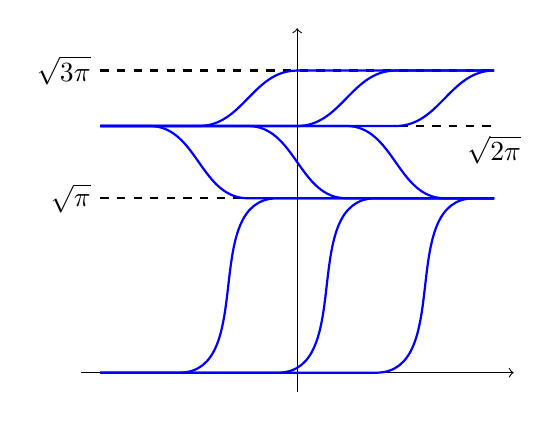
\begin{tikzpicture}[x=1.25cm, y=1.25cm]
            \draw[->] (-2.2, 0) -- (2.2, 0);
            \draw[->] (0, -0.2) -- (0, 3.5);

            \draw[black, thick, dashed] (-2, 1.7724) -- (2, 1.7724);
            \draw[black, thick, dashed] (-2, 2.5066) -- (2, 2.5066);
            \draw[black, thick, dashed] (-2, 3.0699) -- (2, 3.0699);

            \node[anchor=east] at (-2, 1.7724) {\(\sqrt{\pi}\)};
            \node[anchor=east] at (-2, 3.0699) {\(\sqrt{3\pi}\)};
            \node[anchor=north] at (2, 2.5066) {\(\sqrt{2\pi}\)};

            \draw[blue, thick] (-2, 0) -- (-1.2, 0) to[out=0, in=180] (-0.2, 1.7724) -- (2, 1.7724);
            \draw[blue, thick] (-2, 0) -- (-0.2, 0) to[out=0, in=180] (0.8, 1.7724) -- (2, 1.7724);
            \draw[blue, thick] (-2, 0) -- (0.8, 0) to[out=0, in=180] (1.8, 1.7724) -- (2, 1.7724);

            \draw[blue, thick] (-2, 2.5066) -- (-1.5, 2.5066) to[out=0, in=180] (-0.5, 1.7724) -- (2, 1.7724);
            \draw[blue, thick] (-2, 2.5066) -- (-0.5, 2.5066) to[out=0, in=180] (0.5, 1.7724) -- (2, 1.7724);
            \draw[blue, thick] (-2, 2.5066) -- (0.5, 2.5066) to[out=0, in=180] (1.5, 1.7724) -- (2, 1.7724);

            \draw[blue, thick] (-2, 2.5066) -- (-1.0, 2.5066) to[out=0, in=180] (0, 3.0699) -- (2, 3.0699);
            \draw[blue, thick] (-2, 2.5066) -- (0, 2.5066) to[out=0, in=180] (1, 3.0699) -- (2, 3.0699);
            \draw[blue, thick] (-2, 2.5066) -- (1.0, 2.5066) to[out=0, in=180] (2, 3.0699);
        \end{tikzpicture}
\end{center}
    To complete the inverse-curve question, define
    \[
        J=\int_0^\infty h(t)\,dt,\qquad
        x(y)=-\int_y^\infty h(t)\,dt.
    \]
    The integral at infinity is conditionally convergent. Indeed, with \(u=t^2\),
    \[
        J=\frac12\sum_{k=0}^{\infty}(-1)^k A_k,\qquad
        A_k=\int_0^\pi\frac{dv}{\sqrt{k\pi+v}\,(\sin v)^{1/3}}.
    \]
    The numbers \(A_k\) decrease strictly to zero; \(A_0\) is finite since
    its integrand is of order \(v^{-5/6}\) at zero.
    The alternating-series test, with the unfinished last lobe bounded by \(A_k\),
    proves convergence of the improper integral, not just convergence at lobe endpoints.
    Local integrability makes \(x(y)\) continuous through all equilibrium levels.
    Away from them \(x'=h\), so its branches are inverse integral curves.
    Any other such continuous curve differs by a single constant; the limit at
    \(+\infty\) fixes that constant. Since \(h\) is even,
    \[
        \boxed{\lim_{y\to-\infty}x(y)=-2J
        =-\sum_{k=0}^{\infty}(-1)^k
          \int_0^\pi\frac{dv}{\sqrt{k\pi+v}\,(\sin v)^{1/3}}.}
    \]
    This convergent series gives the exact negative value; it is not zero,
    since the strictly decreasing alternating sum is positive.
\end{snippetsolution}


\begin{snippetexercise}{diffeq-quartic-cube-root-exercise}{Finite-time contact and blow-up}
    Study \(y'=x\sqrt[3]{y^4-1}\), \(y(0)=y_0\), using the real cube root.
    Discuss uniqueness and global extendibility for every \(y_0\in\realnumbers\).
\end{snippetexercise}

\begin{snippetsolution}{diffeq-quartic-cube-root-solution}{Classification by the initial level}
    Put \(g(y)=\sqrt[3]{y^4-1}\). The equilibria are \(y=\pm1\);
    \(g>0\) outside \([-1,1]\) and \(g<0\) inside.
    Off those equilibria,
    \[
        \int_{y_0}^{y(x)}\frac{dt}{g(t)}=\frac{x^2}{2}.
    \]
    The endpoint singularities at \(\pm1\) have order \(|t\mp1|^{-1/3}\)
    and are integrable.
    \begin{enumerate}
        \item If \(y_0>1\), the unique even solution blows up at both endpoints
        of \((-T_+,T_+)\), where
        \[
            T_+=\sqrt{2\int_{y_0}^\infty\frac{dt}{\sqrt[3]{t^4-1}}}<\infty,
        \]
        since the integrand is asymptotic to \(t^{-4/3}\).
        \item If \(y_0<-1\), the solution increases outward toward \(-1\),
        reaching it at
        \[
            |x|=\sqrt{2\int_{y_0}^{-1}\frac{dt}{\sqrt[3]{t^4-1}}}.
        \]
        The signs force continuation as \(-1\), giving a unique global solution.
        \item If \(-1<y_0<1\), the same formula with upper limit \(-1\)
        is positive (both orientation and integrand are negative).
        The solution decreases outward, reaches \(-1\), and stays there.
        It is again unique and global.
        \item If \(y_0=-1\), only the constant solution is possible.
        \item If \(y_0=1\), on each half-axis independently one may wait
        at \(1\), depart upward and blow up, or depart downward, reach \(-1\)
        and remain there. Hence there are both global and nonglobal solutions.
    \end{enumerate}
    Thus all data \(y_0<1\) give a unique global solution; data \(y_0>1\)
    give a unique nonglobal solution.
    The two original drawings are retained below. The sign diagram is correct;
    the orange curves in the first drawing below \(-1\) are not solution curves:
    they should approach \(-1\) outward, not descend or blow up.
    Nor can a solution starting at \(-1\) depart outward below it.
\begin{center}
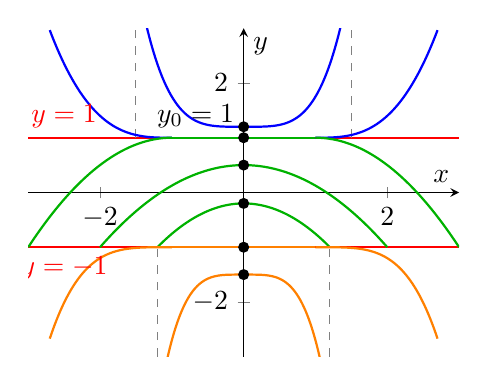
\begin{tikzpicture}
                \begin{axis}[
                        width=10cm,
                        scale=0.65,
                        height=8cm,
                        xmin=-3, xmax=3,
                        ymin=-3, ymax=3,
                        axis lines=middle,
                        xlabel=$x$,
                        ylabel=$y$,
                        samples=100,
                        smooth,
                        clip=true
                    ]

                    \addplot[red, thick, domain=-3:3] {1};
                    \addplot[red, thick, domain=-3:3] {-1};

                    \addplot[blue, thick, domain=-1.5:1.5] {1.2 + 0.55*x^4};
                    \draw[dashed, gray] (axis cs:1.5, 1) -- (axis cs:1.5, 3);
                    \draw[dashed, gray] (axis cs:-1.5, 1) -- (axis cs:-1.5, 3);

                    \addplot[blue, thick, domain=-1:1] {1};
                    \addplot[blue, thick, domain=1:2.7] {1 + 0.4*(x-1)^3};
                    \addplot[blue, thick, domain=-2.7:-1] {1 + 0.4*(-x-1)^3};

                    \addplot[green!70!black, thick, domain=-1:1] {1};
                    \addplot[green!70!black, thick, domain=1:3] {1 - 0.5*(x-1)^2};
                    \addplot[green!70!black, thick, domain=-3:-1] {1 - 0.5*(-x-1)^2};

                    \addplot[green!70!black, thick, domain=-2:2] {0.5 - 0.375*x^2};

                    \addplot[green!70!black, thick, domain=-1.2:1.2] {-0.2 - 0.555*x^2};

                    \addplot[orange, thick, domain=-1:1] {-1};
                    \addplot[orange, thick, domain=1:2.7] {-1 - 0.2*(x-1)^4};
                    \addplot[orange, thick, domain=-2.7:-1] {-1 - 0.2*(-x-1)^4};

                    \addplot[orange, thick, domain=-1.2:1.2] {-1.5 - 1.2*x^4};
                    \draw[dashed, gray] (axis cs:1.2, -3) -- (axis cs:1.2, -1);
                    \draw[dashed, gray] (axis cs:-1.2, -3) -- (axis cs:-1.2, -1);

                    \fill[black] (axis cs:0, 1.2) circle (2pt);
                    \fill[black] (axis cs:0, 1) circle (2pt) node[above left] {$y_0=1$};
                    \fill[black] (axis cs:0, 0.5) circle (2pt);
                    \fill[black] (axis cs:0, -0.2) circle (2pt);
                    \fill[black] (axis cs:0, -1) circle (2pt);
                    \fill[black] (axis cs:0, -1.5) circle (2pt);

                    \node[red, above] at (axis cs:-2.5, 1) {$y=1$};
                    \node[red, below] at (axis cs:-2.5, -1) {$y=-1$};

                \end{axis}
            \end{tikzpicture}
\end{center}
\begin{center}
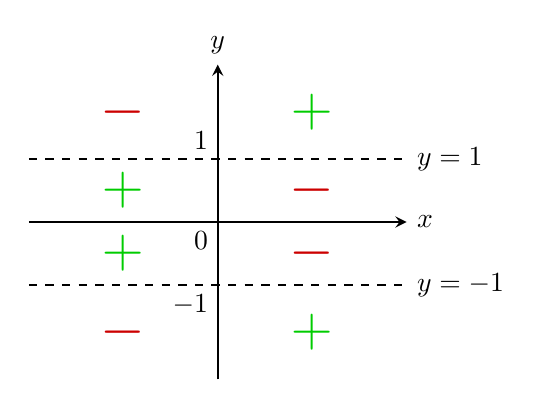
\begin{tikzpicture}[scale=0.8, x=1.2cm, y=1cm, >=stealth]
                \draw[->, thick] (-2.5, 0) -- (2.5, 0) node[right] {$x$};
                \draw[->, thick] (0, -2.5) -- (0, 2.5) node[above] {$y$};

                \draw[dashed, thick] (-2.5, 1) -- (2.5, 1) node[right] {$y=1$};
                \draw[dashed, thick] (-2.5, -1) -- (2.5, -1) node[right] {$y=-1$};

                \node[below left] at (0,0) {$0$};
                \node[above left] at (0,1) {$1$};
                \node[below left] at (0,-1) {$-1$};

                \node[text=green!80!black] at (1.25, 1.75) {\huge $+$};
                \node[text=red!80!black] at (1.25, 0.5) {\huge $-$};
                \node[text=red!80!black] at (1.25, -0.5) {\huge $-$};
                \node[text=green!80!black] at (1.25, -1.75) {\huge $+$};

                \node[text=red!80!black] at (-1.25, 1.75) {\huge $-$};
                \node[text=green!80!black] at (-1.25, 0.5) {\huge $+$};
                \node[text=green!80!black] at (-1.25, -0.5) {\huge $+$};
                \node[text=red!80!black] at (-1.25, -1.75) {\huge $-$};
            \end{tikzpicture}
\end{center}
\end{snippetsolution}
\end{document}
